
\chapter{Retropropagación en capa SoftMax} \label{softmax_apendice}


Tal y como se comentó en secciones anteriores, se empleará SoftMax en la última capa totalmente conectada. De este modo, se definen los valores de entrada a la misma como \textit{Z}, y los de salida como \textit{O}, tal y como se muestra en la Figura \ref{cross_entropy_notacion_apendice}.

\begin{figure}[H]
	\centering
	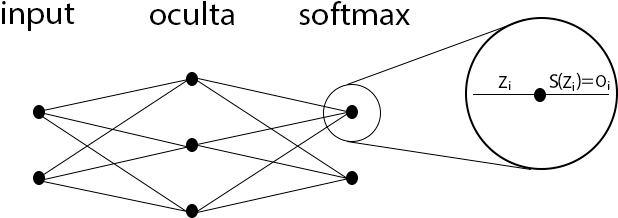
\includegraphics[scale=0.4]{imagenes/NN_softmax.jpg}  
	\caption{Estructura de una red totalmente conectada con softmax en la última capa}
\end{figure}

\begin{gather}
	E = - \sum_{i=1}^{N}  [y_i * ln(O_i)] 
	\label{cross_entropy_notacion_apendice}
\end{gather}

Según esta notación, la función de error \ref{fig:loss_func_softmax} se convierte en la fórmula \ref{cross_entropy_notacion_apendice}.

\section{Cálculo del gradiente de la función de error}

Para comenzar la retropropagación, empezaremos por calcular el gradiente de la función de pérdida con respecto a cada parámetro de entrada de la capa en la cual se aplicó SoftMax, esto se muestra en la fórmula \ref{grad_H_Z}.
\begin{gather}
	\frac{\partial E}{\partial Z_k} = \frac{\partial(- \sum_{i=1}^{H}  [y_i * ln(O_i)])}{\partial Z_k} = - \sum_{i=1}^{H}  [\frac{\partial(y_i * ln(O_i))}{\partial Z_k}] 
	\label{grad_H_Z}
\end{gather}

Como $y_i$ (etiqueta real), es independiente con respecto a $Z_k$ (neurona artificial de entrada), en la fórmula \ref{grad_H_Z}, esta se trata como una constante. \\
\begin{gather}
	\frac{\partial E}{\partial Z_k} = - \sum_{i=1}^{H}  [y_i * \frac{\partial(ln(O_i))}{\partial Z_k}] 
	\label{grad_O_K}
\end{gather}

Por simplificar los cálculos y eliminar el logaritmo de la ecuación, se aplica la regla de la cadena, y, como resultado, se obtienen las fórmulas \ref{gradiente_Oi_Zk_1} y \ref{gradiente_Oi_Zk_2}.
\begin{gather}	
	\frac{\partial E}{\partial Z_k} = - \sum_{i=1}^{H}  [y_i * \frac{\partial(ln(O_i))}{\partial O_i} * \frac{\partial O_i}{\partial Z_k}]
	\label{gradiente_Oi_Zk_1} \\
	\frac{\partial E}{\partial Z_k} = - \sum_{i=1}^{H}  [\frac{y_i}{O_i} * \frac{\partial O_i}{\partial Z_k}] 
	\label{gradiente_Oi_Zk_2}
\end{gather}

% ver https://www.mldawn.com/the-derivative-of-softmaxz-function-w-r-t-z/

\section{Derivada de softmax con respecto a su entrada, $\frac{\partial O_i}{\partial Z_k}$}

Una vez obtenida la fórmula \ref{gradiente_Oi_Zk_2}, nos disponemos a calcular la derivada de $O_i$ con respecto $Z_i$. \\
Sin embargo, hay que contemplar 2 casos posibles, siendo estos $\frac{\partial S(Z_i)}{\partial Z_i}$ y $\frac{\partial S(Z_i)}{\partial Z_j}$, donde i $\neq$ j. \\

\section{Caso $\frac{\partial S(Z_i)}{\partial Z_i}$}

\begin{gather}
	\frac{\partial f(x)}{\partial g(x)} = \frac{f'(x)*g(x) - g'(x)*f(x)}{g(x)^2} \\
	S(z_i) = \frac{e^{Z_i}}{e^{Z_1} + ... + e^{Z_H}} \\
	\frac{\partial S(Z_1)}{\partial Z_1} = \frac{[\frac{\partial e^{Z_1}}{\partial Z_1} * (e^{Z_1} + ... + e^{Z_H}) ] - [\frac{\partial (e^{Z_1} + ... + e^{Z_H})}{\partial Z_1} * e^{Z_1} ] }{(e^{Z_1} + ... + e^{Z_H})^2} 
\end{gather}

Se aplica $\frac{\partial e^{Z_1}}{\partial Z_1} = e^{Z_1}$ \\
\begin{gather}
	\frac{\partial S(Z_1)}{\partial Z_1} = \frac{[e^{Z_1} * \sum_{i=1}^{H}  e^{Z_i}] - [e^{Z_1} * e^{Z_1}]   }{ (\sum_{i=1}^{H}  e^{Z_i})^2} \\
\end{gather}

Se saca factor común $e^{Z_1}$ \\
\begin{gather}
	\frac{\partial S(Z_1)}{\partial Z_1} = \frac{e^{Z_1} ([\sum_{i=1}^{H}  e^{Z_i}] - e^{Z_1})  }{(\sum_{i=1}^{H}  e^{Z_i})^2} \\
	\frac{\partial S(Z_1)}{\partial Z_1} = \frac{e^{Z_1}}{\sum_{i=1}^{H}  e^{Z_i}} * \frac{[\sum_{i=1}^{H}  e^{Z_i}] - e^{Z_1}}{\sum_{i=1}^{H}  e^{Z_i}}
\end{gather}

Se recuerda que $\frac{\sum_{i=1}^{H}  e^{Z_i}}{\sum_{i=1}^{H}  e^{Z_i}} = 1$ y que S($Z_1$) = $ \frac{e^{Z_1}}{\sum_{i=1}^{H}  e^{Z_i}}$ \\
\begin{gather}
	\frac{\partial S(Z_1)}{\partial Z_1} = S(Z_1) * (1- S(Z_1))
	\label{grad_Oi_Zk_drch}
\end{gather}

\subsection{Caso $\frac{\partial S(Z_i)}{\partial Z_j}$, con i $\neq$ j}

\begin{gather}
	\frac{\partial S(Z_2)}{\partial Z_1} = \frac{[\frac{\partial e^{Z_2}}{\partial Z_1} * (e^{Z_1} + ... + e^{Z_H}) ] - [\frac{\partial (e^{Z_1} + ... + e^{Z_H})}{\partial Z_1} * e^{Z_2} ] }{(e^{Z_1} + ... + e^{Z_H})^2} \\
	\frac{\partial S(Z_2)}{\partial Z_1} = \frac{[0 * [\sum_{i=1}^{H}  e^{Z_i}]] - [e^{Z_1} * e^{Z_2}]   }{ (\sum_{i=1}^{H}  e^{Z_i})^2} \\
	\frac{\partial S(Z_2)}{\partial Z_1} = \frac{-e^{Z_1} * e^{Z_2}  }{(\sum_{i=1}^{H}  e^{Z_i})^2} \\
	\frac{\partial S(Z_2)}{\partial Z_1} = \frac{-e^{Z_1}}{\sum_{i=1}^{H}  e^{Z_i}} * \frac{e^{Z_2}}{\sum_{i=1}^{H}  e^{Z_i}} \\
	\frac{\partial S(Z_2)}{\partial Z_1} = -S(Z_1) * S(Z_2)
	\label{grad_Oi_Zk_izq}
\end{gather}

\section{Combinación de casos}

De esta forma, tendremos que dividir  el proceso en 2 partes, cuando i sea igual a j, y cuando i $\neq$ j. \\
Como todos los casos menos uno pertenecen al caso i $\neq$ k, en la fórmula \ref{comb_casos} se aprecia como la ``parte izquierda'' hace referencia al caso i!=k, mientras que la ``parte derecha'' a i=k. \\
Retomamos la fórmula \ref{gradiente_Oi_Zk_2}, aplicando \ref{grad_Oi_Zk_izq} en la parte izquierda, y \ref{grad_Oi_Zk_drch} en la derecha. \\
\begin{gather}
	\frac{\partial E}{\partial Z_k} = - [\sum_{i!=k}^{H} [\frac{y_i}{O_i} * -O_i * O_k ] + \frac{y_k}{O_k} * O_k * (1 - O_k)  ]
	\label{comb_casos}
\end{gather}

Una vez obtenida la fórmula \ref{comb_casos}, se simplifica $O_i$ en la parte izquierda y $O_k$ en la derecha. \\
\begin{gather}
	\frac{\partial E}{\partial Z_k} = - [\sum_{i!=k}^{H} [- y_i * O_k] + [y_k * (1 - O_k) ] ] 
	\label{simplificacion_Oi_Ok}
\end{gather}

Se extrae $O_k$ de la suma en la fórmula \ref{simplificacion_Oi_Ok}, pues es independiente con respecto al índice $i$ y se obtiene la fórmula \ref{simplificar}.\\
\begin{gather}	
	\frac{\partial E}{\partial Z_k} = - [-O_k \sum_{i!=k}^{H}[-y_i] + [y_k * (1 - O_k) ] ]
	\label{simplificar}
\end{gather}

\section{Simplificación One-Hot}

Al emplear la codificación one-hot en Y, se sabe que la suma de sus elementos es igual a 1, pues para un ejemplo de entrada $x_i \in X$, su etiqueta asociada $y_i \in Y$ presenta todos sus valores iguales a 0 menos uno de ellos con el valor de 1. \\
Con estos datos, se calculan las fórmulas \ref{one_hot_simplif_1} y \ref{one_hot_simplif_2}.
\begin{gather}
	\sum_{i=1}^{H} y_i = 1 \label{one_hot_simplif_1}\\
	\sum_{i!=k}^{H} y_i = \sum_{i=1}^{H} [y_i] - y_k = 1 - y_k
	\label{one_hot_simplif_2}
\end{gather}

Una vez obtenidas dichas fórmulas, se emplea \ref{one_hot_simplif_2} para simplificar la suma anterior obtenida en \ref{simplificar}, y, como resultado, se obtienen las fórmulas \ref{one_hot_simplif_3} y \ref{one_hot_simplif_4}. \\


\begin{gather}
	\frac{\partial E}{\partial Z_k} = [O_k*(1-y_k)] - [y_k*(1-O_k)] \label{one_hot_simplif_3} \\
	\frac{\partial E}{\partial Z_k} = O_k - O_k * y_k - y_k + O_k * y_k  \label{one_hot_simplif_4}
\end{gather}

Por último, en la fórmula \ref{one_hot_simplif_4}, se simplifica $O_k*y_k$, y se obtiene la fórmula final \ref{gradiente_softmax_apendice} \cite{Cross_entropy_backprop} \cite{Cross_entropy_backprop_grad_input}. \\
\begin{gather}
	\frac{\partial E}{\partial Z_k} = O_k - y_k = gradiente\_Z_k
	\label{gradiente_softmax_apendice}
\end{gather} 
